%% LyX 2.3.1 created this file.  For more info, see http://www.lyx.org/.
%% Do not edit unless you really know what you are doing.
\documentclass[oneside,english]{extbook}
\usepackage{lmodern}
\renewcommand{\sfdefault}{lmss}
\renewcommand{\ttdefault}{lmtt}
\usepackage[T1]{fontenc}
\usepackage[latin9]{inputenc}
\usepackage{geometry}
\geometry{verbose,tmargin=25mm,bmargin=25mm,lmargin=25mm,rmargin=25mm}
\pagestyle{empty}
\setcounter{secnumdepth}{3}
\setcounter{tocdepth}{3}
\setlength{\parindent}{0bp}
\usepackage{babel}
\usepackage{float}
\usepackage{graphicx}
\usepackage{setspace}
\onehalfspacing
\usepackage[unicode=true,pdfusetitle,
 bookmarks=true,bookmarksnumbered=false,bookmarksopen=false,
 breaklinks=false,pdfborder={0 0 1},backref=false,colorlinks=false]
 {hyperref}

\makeatletter
%%%%%%%%%%%%%%%%%%%%%%%%%%%%%% User specified LaTeX commands.
\usepackage{amssymb}
\usepackage{color}
\usepackage{listings}
\definecolor{hellgelb}{rgb}{1,1,0.85}
\definecolor{colKeys}{rgb}{0,0,1}
\definecolor{colIdentifier}{rgb}{0,0,0}
\definecolor{colComments}{rgb}{1,0,0}
\definecolor{colString}{rgb}{0,0.5,0}
\lstset{
      language=Matlab,
      float=hbp,
      basicstyle=\footnotesize\ttfamily,
      identifierstyle=\color{colIdentifier},
      keywordstyle=\color{colKeys},
      stringstyle=\color{colString},
      commentstyle=\itshape\color{colComments},
      columns=fixed,
      tabsize=4,
      frame=single,
      framerule=1pt,
      extendedchars=true,
      showspaces=false,
      showstringspaces=false,
      numbers=left,
      numberstyle=\tiny\ttfamily,
      numbersep=1em,
      breaklines=true,
      breakindent=10pt,
      backgroundcolor=\color{hellgelb},
      breakautoindent=true,
      captionpos=t,
      xleftmargin=1em,
      xrightmargin=\fboxsep
}
\usepackage{lscape}
\usepackage{amsmath}
\usepackage{pifont}
\usepackage{color}

\delimitershortfall=-1pt
\let\Right\right
\let\Left\left
\makeatletter
\def\right#1{\Right#1\@ifnextchar){\!\right}{}}
\def\left#1{\Left#1\@ifnextchar({\!\left}{}}
\makeatother

\makeatother

\begin{document}
\pagenumbering{gobble}

\begin{landscape}
\begin{center}
\textbf{Robot's coordinates in the global reference frame}
\par\end{center}

\begin{figure}[H]
\centering\includegraphics[scale=0.95]{../FIGURES/fig01}
\end{figure}
\end{landscape}

Given:
\noindent \begin{flushleft}
The robot's initial pose, $\left(x_0, \, y_0, \, \theta_0\right)$,
and the wheels' angular velocities $(\omega_l, \, \omega_r)$, the
following expressions can be derived:\\
\par\end{flushleft}

\begin{align*}
\alpha \, &= \, \omega \, t\\
r \, &= \, \left(Rs \, + \, \frac{W}{2} \right) \, \alpha\\
l \, &= \, \left(Rs \, - \, \frac{W}{2} \right) \, \alpha\\
\dot{r} \, &= \, \left(Rs \, + \, \frac{W}{2} \right) \, \dot{\alpha} \, \longrightarrow \, v_r \, = \, \left(Rs \, + \, \frac{W}{2} \right) \, \omega\\ 
\dot{l} \, &= \, \left(Rs \, - \, \frac{W}{2} \right) \, \dot{\alpha} \, \longrightarrow \, v_l \, = \, \left(Rs \, - \, \frac{W}{2} \right) \, \omega 
\end{align*}

\begin{align*}
\omega \, &= \, \dfrac{v_r \, - \, v_l}{W}\\
Rs \, &= \, \dfrac{v_r \, + \, v_l}{2 \, \omega} \, = \, \dfrac{v}{\omega} \, = \, \dfrac{W}{2} \, \left( \dfrac{v_r \, + \, v_l}{v_r \, - \, v_l} \right)
\end{align*}

Summary:

\begin{align*}
\omega \, &= \, \dfrac{v_r \, - \, v_l}{W}\\
v \, &= \, \dfrac{v_r \, + \, v_l}{2}\\
Rs \, &= \, \dfrac{v}{\omega} \, = \, \dfrac{W}{2} \, \left(\dfrac{v_r \, + \, v_l}{v_r \, - \, v_l}\right)
\end{align*}

Distance travelled by each wheel:

\begin{align*}
D_r \, &= \, r_w \, \phi_r\\
D_l \, &= \, r_w \, \phi_l
\end{align*}

\begin{align*}
\dot{D_r} \, &= \, r_w \, \dot{\phi_r} \, \longrightarrow \, v_r \, = \, r_w \, \omega_r\\
\dot{D_l} \, &= \, r_w \, \dot{\phi_l} \, \longrightarrow \, v_l \, = \, r_w \, \omega_l
\end{align*}

So, finally:

\begin{align*}
\omega \, &= \, \dfrac{v_r \, - \, v_l}{W} \, = \, \dfrac{r_w}{W} \, \left(\omega_r \, - \, \omega_l \right)\\
v \, &= \, \dfrac{v_r \, + \, v_l}{2} \, = \, \dfrac{r_w}{2} \, \left(\omega_r \, + \, \omega_l\right)\\
Rs \, &= \, \dfrac{v}{\omega} \, = \, \dfrac{W}{2} \, \left(\dfrac{v_r \, + \, v_l}{v_r \, - \, v_l}\right)  \, = \, \dfrac{W}{2} \, \left( \dfrac{\omega_r \, + \, \omega_l}{\omega_r \, - \, \omega_l} \right) 
\end{align*}

\begin{align*}
x_l \, &= \, x \, + \, sd \, \cos\left(\theta\right)\\
y_l \, &= \, y \, + \, sd \, \sin\left(\theta\right)
\end{align*}

\begin{align*}
\cos\left(u \, \pm \, v\right) \, = \, \cos u \, \cos v \, \mp \, \sin u \, \sin v\\
\sin\left(u \, \pm \, v\right) \, = \, \sin u \, \cos v \, \pm \, \cos u \, \sin v
\end{align*}

\begin{align*}
\cos\left(u \, - \, v\right) - \cos\left(u \, + \, v\right) \, = \, 2 \, \sin\left(u\right) \, \sin\left(v\right)\\
\sin\left(u \, + \, v\right) - \sin\left(u \, - \, v\right) \, = \, 2 \, \cos\left(u\right) \, \sin\left(v\right)\\
\end{align*}

\begin{align*}
Ch \, = \, 2 \, Rs \, sin\left(\dfrac{\alpha}{2}\right)
\end{align*}

\begin{align*}
x \, &= \, x_0 \, + \, x_{@} \, + \, x_{\#}\\
&= \, x_0 \, + \, x' \, \cos\left(\theta_0\right) \, + \, y' \, \cos\left(\theta_0 \, + \, 90^{\circ}\right)\\
&= \, x_0 \, + \, Ch \, \cos\left(\dfrac{\alpha}{2}\right) \, \cos\left(\theta_0\right) + \, Ch \, \sin\left(\dfrac{\alpha}{2}\right) \, \cos\left(\theta_0 \, + \, 90^{\circ}\right)\\
&= \, x_0 \, + \, Ch \, \cos\left(\dfrac{\alpha}{2}\right) \, \cos\left(\theta_0\right) - \, Ch \, \sin\left(\dfrac{\alpha}{2}\right) \, \sin\left(\theta_0\right)\\
&= \, x_0 \, + \, Ch \, \cos\left(\theta_0 \, + \, \dfrac{\alpha}{2}\right)\\
& = \, x_0 \, + \, 2 \, Rs \, sin\left(\dfrac{\alpha}{2}\right) \, \cos\left(\theta_0 \, + \, \dfrac{\alpha}{2}\right)\\
& = \, x_0 \, + \, Rs \, \left( \sin \left(\theta_0 \, + \, \alpha \right) - \sin \left( \theta_0 \right) \right)
\end{align*}

\begin{align*}
v_x \, = \, \dot{x} \, &= \, Rs \, \omega \, \cos \left(\theta_0 \, + \, \alpha \right)\\
&= \, v \, \cos \left(\theta_0 \, + \, \alpha \right)
\end{align*}

\begin{align*}
y \, &= \, y_0 \, + \, y_{@} \, + \, y_{\#}\\
&= \, y_0 \, + \, x' \, \sin\left(\theta_0\right) \, + \, y' \, \sin\left(\theta_0 \, + \, 90^{\circ}\right)\\
&= \, y_0 \, + \, Ch \, \cos\left(\dfrac{\alpha}{2}\right) \, \sin\left(\theta_0\right) + \, Ch \, \sin\left(\dfrac{\alpha}{2}\right) \, \sin\left(\theta_0 \, + \, 90^{\circ}\right)\\
&= \, y_0 \, + \, Ch \, \cos\left(\dfrac{\alpha}{2}\right) \, \sin\left(\theta_0\right) + \, Ch \, \sin\left(\dfrac{\alpha}{2}\right) \, \cos\left(\theta_0\right)\\
&= \, y_0 \, + \, Ch \, \sin\left(\theta_0 \, + \, \dfrac{\alpha}{2}\right)\\
&=\, y_0 \, + \, 2 \, Rs \, sin\left(\dfrac{\alpha}{2}\right) \, \sin\left(\theta_0 \, + \, \dfrac{\alpha}{2}\right)\\
&=\, y_0 \, + \, Rs \, \left( cos \left( \theta_0 \right) \, - \, \cos \left( \theta_0 \, + \, \alpha \right) \right)
\end{align*}

\begin{align*}
v_y \, = \, \dot{y} \, &= \, Rs \, \omega \, \sin \left(\theta_0 \, + \, \alpha \right)\\
&= \, v \, \sin \left(\theta_0 \, + \, \alpha \right)
\end{align*}

Another way to calculate the robot's coordinates in the global reference
frame:

\begin{align*}
x_c \, &= \, x_0 \, + \, Rs \, \cos \left( \theta_0 \, + \, 90^{\circ} \right)\\
&= \, x_0 \, - \, Rs \, sin \left( \theta_0 \right)\\
y_c \, &= \, y_0 \, + \, Rs \, \sin \left( \theta_0 \, + \, 90^{\circ} \right)\\
&= \, y_0 \, + \, Rs \, \cos \left( \theta_0 \right)\\
\end{align*}

\begin{align*}
x_c \, &= \, x \, + \, Rs \, \cos \left( \theta_0 \, + \, \alpha \, + \, 90^{\circ} \right)\\
&= \, x \, - \, Rs \, sin \left( \theta_0 \, + \, \alpha \right)\\
y_c \, &= \, y \, + \, Rs \sin \left( \theta_0 \, + \, \alpha \, + \, 90^{\circ} \right)\\
&= \, y \, + \, Rs \, \cos\left( \theta_0 \, + \, \alpha \right)\\
\end{align*}

\begin{align*}
x \, &= \, x_c \, + \, Rs \, \sin \left( \theta_0 \, + \, \alpha \right)\\
&= \, x_0 \, - \, Rs \, \sin\left(\theta_0\right) \, + \, Rs \, \sin \left(\theta_0 \, + \, \alpha \right)\\
&= \, x_0 \, + \, Rs \, \left( \sin \left( \theta_0 \, + \, \alpha \right) \, - \, \sin \left( \theta_0 \right) \right)\\
&= \, x_0 \, + \, 2 \, Rs \, \cos\left(\theta_0 \, + \, \dfrac{\alpha}{2}\right) \, \sin\left(\dfrac{\alpha}{2}\right)
\end{align*}

\begin{align*}
y \, &= \, y_c \, - \, Rs \, \cos \left( \theta_0 \, + \, \alpha \right)\\
&= \, y_0 \, + \, Rs \cos \left( \theta_0 \right) - \, Rs \, \cos \left( \theta_0 \, + \, \alpha \right)\\
&= \, y_0 \, + \, Rs \, \left( \cos \left( \theta_0 \right) \, - \, \cos \left( \theta_0 \, + \, \alpha \right) \right)\\
&= \, y_0 \, + \, 2 \, Rs \, \sin\left(\theta_0 \, + \, \dfrac{\alpha}{2}\right) \, \sin\left(\dfrac{\alpha}{2}\right)
\end{align*}

\newpage

For completeness, let's considerate the case when the robot is located
at the pose $\left(x_0, \, y_0, \, \theta_0\right)$ and wants to
get to the pose $\left(x, \, y, \, \theta\right)$, i.e, any pose
known in advanced in the robot's environment. The easiest way to move
between these two points is by describing and arc.

But, what is the turning radius, i.e $Rs$, that allows the robot
to describe that arc?

As the first figure depicts, the initial and final poses are linked
by the chord $Ch$.

\begin{align*}
\Delta x \, &= \, x \, - \, x_0\\
\Delta y \, &= \, y \, - \, x_0\\
Ch^2 \, &= \, {\Delta x}^2 \, + \, {\Delta y}^2 \, = \, x'^2 \, + \, y'^2
\end{align*}

The heading error, i.e, the difference between the chord's angle and
the robot's orientation is:

\begin{align*}
\theta_{err} \, &= \, \dfrac{\alpha}{2} \, = \, \arctan \left( \dfrac{\Delta \, y}{\Delta x} \right) \, - \, \theta_0\\
\end{align*}

So, the turning radius (with sign) $Rs$ can be computed, geometrically,
as:

\begin{align*}
Rs \, &= \, d \, + \, y'\\
Rs^2 \, &= \, d^2 \, + \, x'^2 \, = \, (Rs \, - \, y')^2 \, + \, x'^2
\end{align*}

Also:

\begin{align*}
y' \, &= \, Ch \, \sin \left( \theta_{err} \right)
\end{align*}

Therefore:

\begin{align*}
Rs^2 \, &= \, \left( Rs \, - \, y' \right)^2 \, + \, x'^2 \\
&= \, Rs^2 \, + \, y'^2 \, - \, 2 \, Rs \, y' + x'^2\\
&= \, Rs^2 \, + \, Ch^2 \, - \, 2 \, Rs \,y'\\
Rs \, &= \, \dfrac{Ch^2}{2 \, y'} \, = \, \dfrac{Ch^2}{2 \, Ch \, \sin \left( \theta_{err} \right)} \,= \, \dfrac{Ch}{2 \, \sin \left( \theta_{err} \right)}
\end{align*}

\newpage

\begin{landscape}
\begin{center}
\textbf{Robot's coordinates in the global reference frame}
\par\end{center}

\begin{figure}[H]
\centering\includegraphics[scale=0.95]{../FIGURES/fig02}
\end{figure}
\end{landscape}

Given the robot's initial pose, $\left(x_0, \, y_0, \, \theta_0\right)$,
and the motion commands, $(l, \, r)$:

\begin{align*}
x \,&=\, x_0 \, + \, l \, \cos\left(\theta_0\right)\\
y \,&=\, y_0 \, + \, l \, \sin\left(\theta_0\right)\\
x_l \,&=\, x \, + \, sd \, \cos\left(\theta\right)\\
y_l \,&=\, y \, + \, sd \, \sin\left(\theta\right)
\end{align*}
\end{document}
